\subsection{Boosting Short Antennas: The Magic of Loading Coils!}
\begin{tcolorbox}[colback=gray!10, colframe=black, title=E9D09]
What is the function of a loading coil in an electrically short antenna?
\begin{enumerate}[label=\Alph*.]
    \item To increase the SWR bandwidth by increasing net reactance
    \item To lower the losses
    \item To lower the Q
    \item \textbf{To resonate the antenna by cancelling the capacitive reactance}
\end{enumerate} \end{tcolorbox}

\subsubsection{Related Concepts}
In radio communication, electrically short antennas are antennas that are smaller than half the wavelength of the frequencies they are intended to transmit or receive. These antennas typically exhibit a significant amount of capacitive reactance, which can result in poor impedance matching with the transmission line and lead to inefficiencies in radiating energy.

A loading coil serves a crucial role in modifying the electrical characteristics of an electrically short antenna. By adding inductance to the antenna circuit, the loading coil can help to cancel out the capacitive reactance that is inherent in short antennas. This creates a condition where the antenna can resonate, thereby improving its overall performance.

To understand the concept from a mathematical perspective, we recall that the impedance \( Z \) of an antenna is given by:

\[
Z = R + jX
\]

where \( R \) represents the real part (resistance), and \( jX \) represents the imaginary part (reactance).

When a loading coil is introduced, it adds inductive reactance \( jX_L \) to the system. The reactance of the loading coil is given by:

\[
X_L = 2 \pi f L
\]

where \( f \) is the frequency of operation, and \( L \) is the inductance of the coil.

The combined reactance of the antenna with the coil becomes:

\[
X_{total} = X_{antenna} + X_L
\]

To achieve resonance, we set the total reactance \( X_{total} \) to zero:

\[
X_{antenna} + X_L = 0 \implies X_L = -X_{antenna}
\]

This equation illustrates how the loading coil cancels the capacitive reactance of the antenna, allowing it to resonate effectively.

\subsubsection{Diagram of Antenna with Loading Coil}
\begin{center}
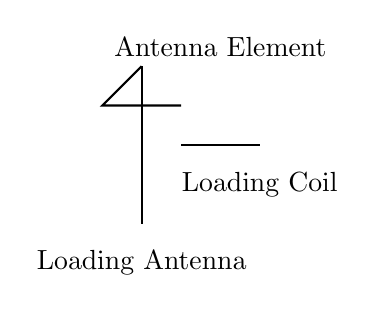
\begin{tikzpicture}
    % Draw the antenna
    \draw[thick] (0,0) -- (0,2);
    \draw[thick] (0,2) -- (-0.5,1.5) -- (0.5,1.5);
    \node at (0,-0.5) {Loading Antenna};

    % Draw the loading coil
    \draw[thick] (1,1) to [out=0, in=180] (1.5,1);
    \draw[thick] (1,1) to [out=180, in=0] (0.5,1);

    % Labels
    \node at (1.5, 0.5) {Loading Coil};
    \node at (1, 2.25) {Antenna Element};
\end{tikzpicture}
\end{center}

In conclusion, 
